\documentclass[11pt]{article}
\usepackage{listings} % Required for Code
\usepackage[left = 1cm, right = 1cm, top = 1cm, bottom = 1cm]{geometry} % Set margins
\usepackage{amsmath} % Required for Writing Mathematics
\usepackage{amssymb} % Contains some mathematical symbols
\usepackage{amsthm}
\usepackage{mathtools}
\DeclarePairedDelimiter\ket{\lvert}{\rangle}
\usepackage{amsfonts} % Contains some mathematical fonts
\usepackage{siunitx}
\usepackage{float} % you insert figures into "floats"
\usepackage{subcaption}
\usepackage[skip=2pt,font=scriptsize]{caption} % added captions
\usepackage{graphicx}

\setlength{\parindent}{0pt} % no paragraph indent
\setlength{\parskip}{\medskipamount} % changes paragraph skip
\title{Electromagnetic Waves - Adil Hashlamon - 6813102}
\author{Adil Hashlamon}
\date{December 2024}
\begin{document}
\underline{\textbf{Example Sheet 1 Worked Solutions}}

\underline{Question 1}

\textit{Question.} Establish Stirling's Formula: $N \approx \sqrt{2\pi N }N^N e^{-N}$

\begin{proof}
We are first given $\int\limits_{0}^{\infty}e^{-x} x^N dx = \int\limits_{0}^{\infty}e^{-F(x)} dx$ and since the integrands are equal, we can equate:
\begin{equation}
    \begin{aligned}
        e^{-x}x^N &= e^{-F(x)} \\
        \Rightarrow F(x) &= x - N\ln x.
    \end{aligned}
\end{equation}

We then differentiate twice in order to find the approximation $F(x) \approx F(x_0) + F''(x_0) (x-x_0)^2/2$ where $x_0$ is $x$ value of the minimum of $F(x)$.
\begin{equation}
    \begin{aligned}
        F'(x) &= 1- \frac{N}{x} \\
        F''(x) &= \frac{N}{x^2}.
    \end{aligned}
\end{equation}

The minimum occurs when $F'(x)=0$ which implies $x_0 = N$ (we assume this is a minimum as it is the only solution to $F'(x)=0$ and the question asks us to find a minimum).

We know have all the information required to determine the approximation and can substitute into the 2nd integral given:

\begin{equation}
    F(x) \approx -N + N \ln  N - \frac{(x-N)^2}{2N}
\end{equation}

\begin{equation}
    \begin{aligned}
        N! &= \int\limits_{0}^{\infty} \exp\left(-N + N \ln  N - \frac{(x-N)^2}{2N}\right) dx \\
        & = e^{-N} N^N \int\limits_{0}^{\infty} \exp\left( - \frac{(x-N)^2}{2N}\right) dx.
    \end{aligned}
\end{equation}

The time has come to apply the final approximation alluded to in the question. The term $x-N$ is effectively shifting the function to the right hand side of the y-axis. And since $N$ is very large, the limits of the integral guarantee that we are integrating the entire curve as it tails to $0$ at either end. \textit{Note: }The factor of $1/2N$ does nothing to affect this shifting.

\begin{figure}[H]
\centering 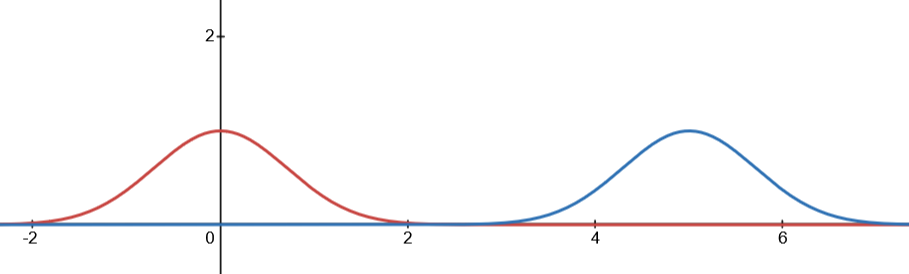
\includegraphics[scale=0.7]{Question 1.1.png} \label{fig:FFTgen}
\caption{Graph of $e^{-x^2}$ in red vs $e^{-(x-5)^2}$ in blue}
\end{figure}
\newpage
Thus, we make the approximation:
\begin{equation}
    N! \approx e^{-N} N^N \int\limits_{-\infty}^{+\infty} \exp\left(\frac{-x^2}{2N}\right) dx.
\end{equation}

As this is the standard form of the Gaussian Integral:
\begin{equation}
    \int\limits_{-\infty}^{+\infty}e^{-ax^2} dx = \sqrt{\frac{\pi}{a}}.
\end{equation}

Thus, with $a= 1/2N$, we have:

\begin{equation}
    N! \approx \sqrt{2\pi N} N^N e^{-N}
\end{equation}
    
\end{proof}


\underline{Question 2i}

\textit{Question.} For a two coupled system in the microcanonical ensemble, show that they maximise their entropy if the heat capacity, $C$, is positive.

\begin{proof}
Considering the system as a whole to have entropy $S$ and equal temperature $T$, we have the equation:
\begin{equation}
    \frac{\partial^2S}{\partial E^2} = -\frac{1}{T^2C}
\end{equation}
If we want the system to have a maximum entropy, the equation on the right hand side must be negative and thus $C$ must be positive.

\end{proof}

\underline{Question 2ii}

\textit{Question.} Show that the energy fluctuations $\triangle E^2 = \langle E^2 \rangle - \langle E\rangle ^2$ are proportional to $C_V$ in the canonical ensemble.


\begin{proof}
    The fluctuations in the canonical ensemble can be written as: 
    \begin{equation}
        \triangle E^2 = - \frac{\partial \langle E \rangle}{\partial \beta}
    \end{equation}
    The definition of the heat capacity $C_V$ in this case is given as: 
    
    \begin{equation}
        \begin{aligned}
            C_V &= \left(\frac{\partial \langle E \rangle}{\partial T} \right)_V \\
            \Rightarrow \partial \langle E \rangle &= C_V \cdot \partial T \\
            \Rightarrow \triangle E^2 &= - C_V \cdot \frac{\partial T}{\partial \beta}
        \end{aligned}
    \end{equation}
    where the subscript denotes that the volume is constant.

    By definition:
    \begin{equation}
            \begin{aligned}
                \beta &= \frac{1}{k_BT}, T\neq 0 \\
                \Rightarrow \frac{\partial \beta}{\partial T} &= - \frac{1}{k_BT^2} \\
                \Rightarrow \frac{\partial T}{\partial \beta} &= -k_BT^2, T\neq 0 \\
                \Rightarrow \triangle E^2 &= C_V k_B T^2, T \neq 0
            \end{aligned}
    \end{equation}
    
\end{proof}
\newpage

\underline{Question 2iii}

\textit{Question.} Show that the Gibbs entropy from the canonical ensemble can be written as 
\begin{equation}
    S = k_B \frac{\partial}{\partial T}(T\ln Z)
\end{equation}
\begin{proof}
    The entropy in the canonical system, derived using the standard definition of $S$ and Stirlings formula is given as:
    \begin{equation}
        S = - k_B \sum_n p(n) \ln p(n).
    \end{equation}

    The probability of the system being in a state $\ket{n}$ is given by the Boltzmann distribution:
    \begin{equation}
        p(n)= \frac{e^{-\beta E_n}}{Z}
    \end{equation}

    Substituting into our form of S:
    \begin{equation}
        \begin{aligned}
            S &= -k_B \sum_n \frac{e^{-\beta E_n}}{Z} \ln \left(\frac{e^{-\beta E_n}}{Z}\right) \\
            &= - k_B \sum_n \frac{e^{-\beta E_n}}{Z} \left[-\beta E_n - \ln Z\right] \\
            &= k_B \sum_n \frac{\beta E_ne^{-\beta E_n}}{Z} + \frac{e^{-\beta E_n}}{Z} \ln Z \\
            &= k_B \left[ \sum_n \frac{\beta E_n}{Z} e^{-\beta E_n} + \ln Z\right],
        \end{aligned}   
    \end{equation}
Where the last step is made as $\sum_n e^{-\beta E_n}/Z = \sum_n p(n) =1$ as something must happen.

Now, we work backwards from the Gibbs entropy:
\begin{equation}
    \begin{aligned}
        S &= k_b \frac{\partial}{\partial T} (T \ln Z) \\
        & = k_B \left[T \cdot \frac{1}{Z} \cdot \frac{\partial Z}{\partial T} + \ln Z\right]
    \end{aligned}
\end{equation}

$Z$ is given as: 
\begin{equation}
    \begin{aligned}
        Z &= \sum_n e^{-\beta E_n} \\
        &= \sum_n e^{-E_n/k_BT}
    \end{aligned}
\end{equation}

Differentiating with respect to T:
\begin{equation}
    \begin{aligned}
        \frac{\partial Z}{\partial T} &= \sum \frac{\partial}{\partial T} (e^{-E_n/k_BT})\\
        &= \sum_n \frac{\partial }{\partial T} \left(- \frac{E_n}{k_BT} \right)e^{- E_n/k_B T}\\
        &= \sum_n \frac{E_n}{k_B T^2} e^{-E_n/k_BT} \\
        &= \sum_n \frac{E_n}{k_B T^2} e^{-\beta E_n}.
    \end{aligned}
\end{equation}
\newpage
We can now substitute this into the Gibbs entropy equation:
\begin{equation}
    \begin{aligned}
        S &= k_B \left[\frac{T}{Z} \sum_n \frac{E_n}{k_B T^2} e^{-\beta E_n} + \ln Z\right] \\
        &= k_B \left[ \sum_n \frac{\beta E_n}{Z} e^{-\beta E_n} + \ln Z\right].
    \end{aligned}
\end{equation}
\end{proof}
\end{document}